\section{Gaussian Pyramid}

The implementation of the Gaussian pyramid follows the next structure:

\begin{lstlisting}[language=python][h!]
class gaussian_pyramid:
    pyramid = []
    '''
    Initialize the pyramid based on an base image, the number of 
    level and a kernel (Gaussian kernel is the default)
    '''
    def __init__(self, img, levels, kernel = None, gauss_kernel_par= 0.3):
    '''
    interpolates the missing information
    '''
    def interpolation(self,x,y,v, interp = 'bilinear'):
	'''
    upsamples an image, using the desired interpolation method
    '''
    def up_sample(self, image, size, interp = 'bilinear'):
    '''
    downsamples an image, using the desired padding strategy
    '''
    def down_sample(self, image, size, padding_type = 'mirror', 
	'''
    Implements the down operation of the pyramid using the upsample function
    '''
    def down(self, level):
	'''
    Implements the up operation of the pyramid using the downsample function
    '''
    def up(self, level): #downsample the image
    '''
    builts the whole pyramid using up function
    '''
    def build(self):
    '''
    returns the desired level of the pyramid
    '''
    def get(self, level):
    '''
    plots each pyramid level
    '''
    def show(self, name = 'gauss_pyramid'):
\end{lstlisting}

We decided this architecture because it needs to compute each level of the pyramid just once, this is useful when function $get$ is implement recovering each level in $O(1)$, in the same way, this implementation is more transparent for an user, allowing easy and fast use of the pyramid as shown below. 

\begin{lstlisting}[language=python][h!]
pyramid = gaussian_pyramid(img, levels = 7)
pyramid.build()
\end{lstlisting}

Some details of the implementation includes: it can handle multichannel and grayscale images indifferently, it implements only bilinear interpolation\footnote{Based on \url{http://supercomputingblog.com/graphics/coding-bilinear-interpolation/}}, the $down$ function may not return an image of the size of the original one whenever the height or width of the image is odd.

The results of the applying the $up$ function to built the pyramid are shown in figure \ref{fig:gaussian_pyramid}

\begin{figure}[h!]
\centering
  \centering
  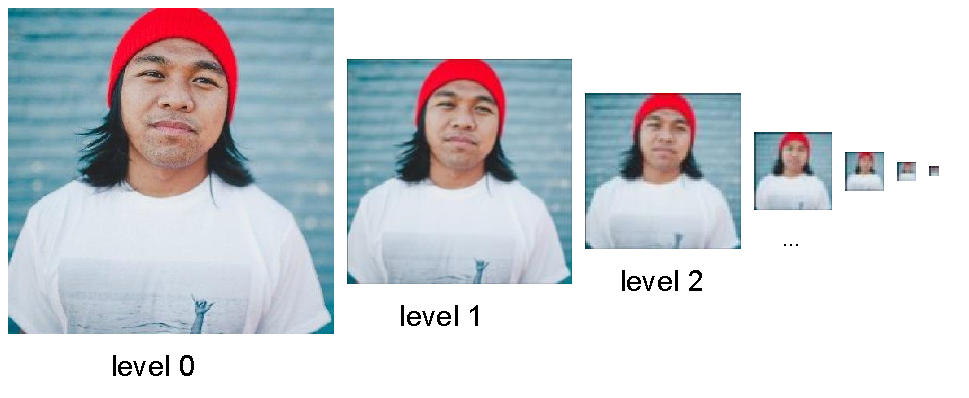
\includegraphics[width=0.9\linewidth]{output/gaussianPyramid.pdf}
  \caption{Gaussian Pyramid}
\label{fig:gaussian_pyramid}
\end{figure}

The result of the $down$ function comparing with the original pyramid level are shown in figure \ref{fig:down-gauss-results}. It can be seen that the upsampled image is not equal to the original one, there is a lost of information that is not recoverable.

\begin{figure}[!h]
\centering
\begin{subfigure}{0.5\textwidth}
  \centering
  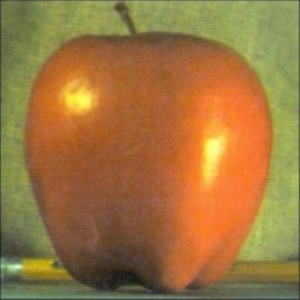
\includegraphics[width=0.8\linewidth]{input/p1-1-3.png}
  \caption{Original image}
\end{subfigure}%
\begin{subfigure}{0.5\textwidth}
  \centering
  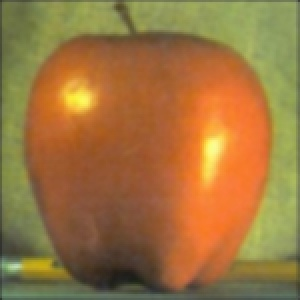
\includegraphics[width=0.8\linewidth]{output/upSample.jpg}
  \caption{Up sampled image}
\end{subfigure}%
 \caption{Comparison of results of $down$ function}
\label{fig:down-gauss-results}
\end{figure}

\section{Laplacian Pyramid}

Similar to Gaussian Pyramid, the implementation of the Laplacian Pyramid, follows the next model:

\begin{lstlisting}[language=python][h!]
class laplacian_pyramid:
    pyramid = []
    '''
    Initialize the pyramid based on the last level of gaussian 
    pyramid,the number of levels and a kernel are of the gaussian
    pyramid
    '''
    def __init__(self, img, levels, kernel = None, gauss_kernel_par = 0.3):  
    '''
    Addition or subtraction an image of level "i" of the gaussian 
    pyramid with the upsampled image of the level i+1 
    '''
    def gauss_operation(self, gauss_cur, gauss_down, operation = '-'):
	'''
    upsamples an image with the down function of the gaussian pyramid
    '''
    def up_sample(self, image, size):
    '''
    upsample an image of a level i of the laplacian pyramid and 
    adds the image of level i+1 of the gaussian pyramid, obtaining 
    the images of the level i of the gaussian pyramid
    '''
    def down(self, up_level_img, cur_level_img):
    '''
    Implements the up operation of the pyramid using the downsample 
    function, this function allows us create one level the 
    laplacian pyramid
    '''
    def up(self, level, gaussian_pyramid):
    '''
    builts the whole pyramid using down function
    '''
    def build(self):  
    '''
    Reconstruct the original image using the laplacian pyramid
    '''
    def reconstruct(self):
    '''
    returns the desired level of the pyramid
    '''
    def get(self, level):
    '''
    plots each pyramid level
    '''
    def show(self, name = 'laplace_pyramid'):
      
\end{lstlisting}

As in the Gaussian implementation, we choose this architecture in order to compute each level of the pyramid just once, this be useful in the blending implementation.

Some details of the implementation includes: it can handle multichannel and grayscale images indifferently, the function  $gauss_operation$ can handle the cases where the upsampled image does not have the same shape as the current level, the $down$ function up samples an image and sum it with another image, this function is the core the the $reconstruct$ function. The last level is equal in the Laplacian pyramid   and Gaussian pyramid.

The logic to reconstruct the image is shown in figure \ref{fig:reconstruction-laplace}, initially, the last level $i$ of the Laplacian pyramid is upsampled, and then is added to the level $i-1$, the first row of figure \ref{fig:reconstruction-laplace} shows the elements inside the Laplacian pyramid, the second row shows the intermediate results of upsampling an image that was previously added with the corresponding Laplace pyramid level. Note that the results of the sum up (third row in figure \ref{fig:reconstruction-laplace}) are more clean an look like the original image.

\begin{figure}[h!]
\hspace{-1cm}
  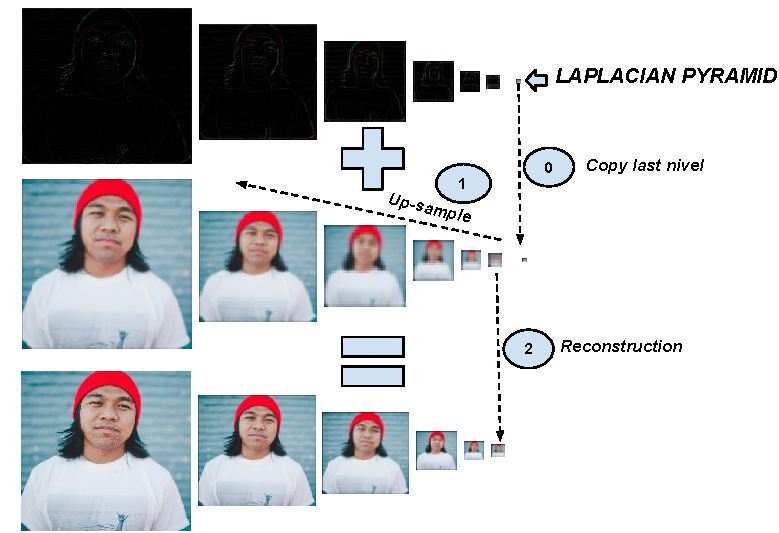
\includegraphics[width=1.1\linewidth]{output/reconstructionImage.pdf}
  \caption{Reconstruction process}
\label{fig:reconstruction-laplace}
\end{figure}
